\subsection{题目描述}
The 24-point game is one of the main puzzle games we played as a child.
The game involves drawing four cards from a deck of playing cards and using any of the operations addition, subtraction, multiplication, and division on the four cards to make the result 24.
For example, using the numbers 2, 3, 4, and 6, the calculation $(((4+6)-2)*3)=24$ yields 24, and the fastest to figure it out wins. Please use Fortran90 programming to solve the solutions for the 24-point game.
\subsection{程序描述}
本题作为递归回溯基本功的经典考题(\href{https://leetcode.com/problems/24-game/description/}{LeetCode $679$}),兼具考察算法知识与编程语言掌握情况的双重作用。
递归回溯最暴力的思路是:从给定的$n$个数中有序取2个数进行四则运算,得到8种运算结果与剩余元素组成8种新的序列,然后对新序列递归调用自身,直到序列中只剩下一个数,判断是否为$24$。不难发现,这样的路径数为
\[
    T_1(n) = 8^{n-1} \binom{n}{2} \binom{n-1}{2}\cdots \binom{2}{2} = 4^{n-1} \cdot n!(n-1)!
\]
对于$T_1(4)=9216$,搜索空间尚可接受,若是$n$再大些,不剪枝实在难受。

第一个朴素的想法是借助表达式树,即$n$个数作为$n$片叶子的二叉树结构种类,可以用$Catalan$数$C_n$表示。更具体说,为$n-1$个运算符所连接的$n$个数表达式添加括号,构成的合法表达式种数为
\[
    C_{n-1}=\binom{2n-2}{n-1} /n.
\]
\newpage
例如,对于$n=4$,$C_3=5$:
\[
    (a \mathbin{\text{op1} \,} (b \mathbin{\text{op2} \,} (c \mathbin{\text{op3} \,} d))), \quad
    (a \mathbin{\text{op1} \,} ((b \mathbin{\text{op2} \,} c) \mathbin{\text{op3} \,} d))
\]
\[
    ((a \mathbin{\text{op1} \,} b) \mathbin{\text{op2} \,} (c \mathbin{\text{op3} \,} d)), \quad
    ((a \mathbin{\text{op1} \,} (b \mathbin{\text{op2} \,} c)) \mathbin{\text{op3} \,} d), \quad
    (((a \mathbin{\text{op1} \,} b) \mathbin{\text{op2} \,} c) \mathbin{\text{op3} \,} d)
\]

\vspace{5pt} % Horizontal space

\begin{forest}
    for tree={
    circle, draw,
    font=\sffamily\large,
    minimum size=2em, inner sep=2pt, s sep=12pt
    }
    [op1
        [a]
        [op2
                [b]
                [op3
                        [c]
                        [d]
                ]
        ]
    ]
\end{forest}
\hspace{5pt} % Horizontal space
\begin{forest}
    for tree={
    circle, draw,
    font=\sffamily\large,
    minimum size=2em, inner sep=2pt, s sep=12pt
    }
    [op1
        [a]
        [op3
                [op2
                        [b]
                        [c]
                ]
                [d]
        ]
    ]
\end{forest}
\hspace{5pt} % Horizontal space
\begin{forest}
    for tree={
    circle, draw,
    font=\sffamily\large,
    minimum size=2em, inner sep=2pt, s sep=12pt
    }
    [op2
        [op1
                [a]
                [b]
        ]
        [op3
                [c]
                [d]
        ]
    ]
\end{forest}
\hspace{5pt} % Horizontal space
\begin{forest}
    for tree={
    circle, draw,
    font=\sffamily\large,
    minimum size=2em, inner sep=2pt, s sep=12pt
    }
    [op3
        [op1
                [a]
                [op2
                        [b]
                        [c]
                ]
        ]
        [d]
    ]
\end{forest}
\hspace{5pt} % Horizontal space
\begin{forest}
    for tree={
    circle, draw,
    font=\sffamily\large,
    minimum size=2em, inner sep=2pt, s sep=12pt
    }
    [op3
        [op2
                [op1
                        [a]
                        [b]
                ]
                [c]
        ]
        [d]
    ]
\end{forest}

\vspace{5pt} % Vertical space
再考虑$n$个数的全排列与各个数之间的运算符种类,可以得到总路径数
\[
    T_2(n) = 4^{n-1} \cdot n! \cdot C_{n-1} = 4^{n-1} \cdot n! \cdot \binom{2n-2}{n-1} /n = 4^{n-1} \cdot (2n-2)!/(n-1)!
\]
对于$T_2(4)=7680$,搜索空间已经减少。

另一种剪枝策略是从加法和乘法的交换律入手,即挑选两个数进行四则运算时,实际上只要考虑$6$种运算结果,这可以将路径数目降至$T_3(n)=3^{n-1} \cdot n!(n-1)!$,对于$T_3(4)=3888$,搜索空间更小。但考虑到两个阶乘复杂度的后发优势,$n=8$时$T_3(8) \approx 4\times10^{11} > T_2(8) \approx 3\times10^{11}$.

自然还会联想到使用分治法,且对于4个数的运算,可以先挑选出一个与24进行四则逆运算,再与前述$n-1$个数的运行结果进行对比,这样的"路径数"为$T_3(n) = n \cdot 4 \cdot T_{2}(n-1) = 4 \cdot 3^{n-1} \cdot (n!)^2$,对于$T_3(4)=1296$,"路径数"的确更少,但考虑到查找比对的开销,实际不一定划算。

本程序最终设计为允许用户最多输入$8$张牌,允许输入整数或者A/J/Q/K(含小写),综合考虑复杂度与Fortran特性,采用了第3种剪枝策略。对于结果的输出,可以将所有解存储再一并输出,但这涉及到未知数目的存储,且在$n>4$时极大影响运行效率(多个数的运算更有可能在较浅搜索区域寻找到解并提前结束),最终决定只输出第一个找到的解。不过 \texttt{game24\_ultra.f90}中,对$n\ge 6 $引入了进度条与\texttt{OpenMP}多线程并行优化,可能同时输出不止一个解。

判断结果正误的精度最初设置为$1 \times 10^{-6}$
,比Fortran内置的单精度\texttt{epsilon(1.0)}大些,但仍不能正确判定$8/(3-8/3) = 24$,便放宽为了$1 \times 10^{-4}$,对于4个$[1,13]$的运算尚未发现误判,但在更大规模的测试中已经发现漏洞,且转为双精度的运算开销实在过大,故在最终结果输出时加注括号与机器运算值,供用户自行检验。

\texttt{./Codes/Problem 2}中有\texttt{game24\_promax.f90}与\texttt{game24\_ultra.f90}两个版本,下文的代码分析以前者为例,后者仅是在GPT o1建议下引入了多线程优化与进度条(实现原理为:提前存储$n=6,7,8$路径数,与已调用次数进行比对)。多线程优化在无解情况测试中被验证是显著有效的。在终端进入其目录,分别运行

\noindent \Colorbox{cmdbg}{\lstinline[language=bash]|gfortran game24_promax.f90 -o promax_test|}、\Colorbox{cmdbg}{\lstinline[language=bash]|gfortran -O -fopenmp game24_ultra.f90 -o ultra_test|}


\noindent 可以编译运行。文件夹中还有\texttt{game24\_promax.exe}与\texttt{game24\_ultra.exe},在大多数Windows系统下可以直接运行。如果是\texttt{x86\_64}架构,建议使用\texttt{\_x64.exe}版本.为了达到最优的运行速度,\textbf{建议使用}

\noindent \Colorbox{cmdbg}{\lstinline[language=bash]|gfortran -O3 -march=native -fopenmp game24_ultra.f90 -o ultra_local|} 命令编译\texttt{Ultra}的本地版本,但在移植到其它架构时可能性能下降。

\subsection{伪代码}
\noindent 主程序与用户交互,调用\texttt{\textbf{Recursive Subroutine solve\_24}},而\texttt{ create\_new\_arrays}生成下一轮数字与表达式。

\vspace{5pt} % Vertical space
\begin{algorithm}[H]
    \caption{Main Program: game24\_promax}
    \label{alg:game24_promax}
    \KwIn{$n$: int, $a$: Array(float, len=n)}
    \KwOut{$sol$: bool}

    \Repeat{\texttt{play\_again} $\ne$ 'y' \textbf{and} $\ne$ 'Y'}{
        \Repeat{$1 \leq n \leq max\_limit$}{
            \Read{$n$}{\tcp*[r]{Enter number of cards between 1 and max\_limit}}
        }
        \Allocate{numbers, expressions}\tcp*[r]{Allocate memory for arrays}
        \For{$i \gets 1$ \textbf{to} $n$}{
            \Read{$\texttt{a[i]}$}{\tcp*[r]{Enter card value $i$}}
            \Call{convert\_to\_number}\tcp*[r]{Convert card to number}
            \Write{expressions[i], numbers[i]}\tcp*[r]{Store as string}
            \Call{remove\_decimal\_zeros}\tcp*[r]{Clean up decimal}
        }
        \texttt{sol} $\gets$ \False\;
        \Call{solve\_24}\tcp*[r]{Solve the 24-point game}
        \If{\texttt{sol} == \False}{\Print{No solution found.}\;}
        \Deallocate{numbers, expressions}\tcp*[r]{Deallocate memory}
        \Read{play\_again} \tcp*[r]{Play again? (y/n)}
    }
\end{algorithm}
\begin{algorithm}[H]
    \caption{Subroutine: create\_new\_arrays}
    \label{alg:create_new_arrays}
    \KwIn{$\texttt{nums}$: Array(float), $\texttt{exprs}$: Array(string), $\texttt{idx1, idx2}$: int, $\texttt{result}$: float, $\texttt{new\_expr}$: string}
    \KwOut{$\texttt{new\_nums}$: Array(float), $\texttt{new\_exprs}$: Array(string)}

    $n \gets$ \texttt{size(nums)}\tcp*[r]{Get the size of input arrays}
    \Allocate{$\texttt{new\_nums}(n - 1), \texttt{new\_exprs}(n - 1)$}\tcp*[r]{Allocate memory for new arrays}

    $j \gets 0$\;
    \For{$i \gets 1$ \textbf{to} $n$}{
        \If{$i \neq \texttt{idx1}$ \textbf{and} $i \neq \texttt{idx2}$}{
            $j \gets j + 1$\;
            $\texttt{new\_nums}(j) \gets \texttt{nums}(i)$\tcp*[r]{Copy remaining numbers}
            $\texttt{new\_exprs}(j) \gets \texttt{exprs}(i)$\tcp*[r]{Copy remaining expressions}
        }
    }

    $\texttt{new\_nums}(n - 1) \gets \texttt{result}$\tcp*[r]{Add result to new arrays}
    $\texttt{new\_exprs}(n - 1) \gets \texttt{new\_expr}$\tcp*[r]{Add new expression to new arrays}
\end{algorithm}

\noindent 程序的核心逻辑是下面的\texttt{\textbf{Recursive Subroutine solve\_24}},

\begin{algorithm}[H]
    \caption{Recursive Subroutine: solve\_24}
    \label{alg:solve_24}
    \KwIn{$nums$: Array(float, len=n), $exprs$: Array(string, len=n), $found$: bool}
    \KwOut{$found$: bool}

    $n \gets \texttt{size}(nums)$\tcp*[r]{Get the size of the array}

    \If{$found$}{\Return\tcp*[r]{If solution is already found, exit recursion}}

    \If{$n = 1$ \textbf{and} \texttt{abs}($nums[1] - 24.0) < 1 \times 10^{-4}$}{
        \Print{Solution found: $exprs[1]$, set $found \gets$ \True}\tcp*[r]{Base case: check if number equals 24}
        \Return\;
    }

    \For{$i \gets 1$ \textbf{to} $n - 1$}{
    \For{$j \gets i + 1$ \textbf{to} $n$}{
        $a, b \gets nums[i], nums[j]$\;
        $expr\_a, expr\_b \gets exprs[i], exprs[j]$\tcp*[r]{Get numbers and their expressions}

        \For{$op \in \{+,-,*,/\}$}{
            \If{$op = /$ \textbf{and} \texttt{abs}($b) < 1 \times 10^{-6}$}{\Continue\tcp*[r]{Skip division by zero}}

            $result \gets a \ op \ b$\tcp*[r]{Apply operator on $a$ and $b$}
            $new\_expr \gets (\texttt{trim}(expr\_a) + op + \texttt{trim}(expr\_b))$\tcp*[r]{Build new expression}

            \Call{create\_new\_arrays}\tcp*[r]{Update arrays with $i$, $j$, result, and new expression}
            \Call{solve\_24($new\_nums, new\_exprs, found$)}\tcp*[r]{Recursive call with updated arrays}
            \If{$found$}{\Return\;}

            \If{$op \in \{-, /\}$ \textbf{and} ($op \neq /$ \textbf{or} \texttt{abs}($a) \geq 1e-6$)}{
                    $result \gets b \ op \ a$\tcp*[r]{Apply reverse operation}
                    $new\_expr \gets (\texttt{trim}(expr\_b) + op + \texttt{trim}(expr\_a))$\;

                    \Call{create\_new\_arrays}\tcp*[r]{Update arrays with $i$, $j$, result, and new expression}
                    \Call{solve\_24($new\_nums, new\_exprs, found$)}\tcp*[r]{Recursive call with reverse operation}
                    \If{$found$}{\Return\;}
                }
            }
        }
    }
\end{algorithm}

\texttt{convert\_to\_number,remove\_decimal\_zeros}仅用于输入输出格式化处理,原理简单,具体实现不再赘述。下面给出一些输入输出实例。

\subsection{输入输出实例}
对于本程序,用户需要先输入牌数$n \in [1,8]$,再输入$n$张牌,可以是整数或者A/J/Q/K(含小写)。程序会输出第一个找到的解\texttt{Solution found:xxx = 24(24.000xxxx)},如果没有解则输出\texttt{No valid solution found.},之后程序会询问是否继续,输入\texttt{Y}或\texttt{y}则继续,否则退出。过程中任何错误输入会被拒绝并要求重新输入。在\texttt{Ultra}版本中,若$n \ge 6$则会启用多线程优化并显示进度条,每$1\%$更新一次进度条。下列表格为在相应输入的计算结果

\begin{table}[ht!]
    \begin{center}
        \begin{tabular}{|c|c|c|c|}\hline
                       & \multicolumn{2}{|c|}{Input} & \multicolumn{1}{|c|}{Output}                                                                  \\\hline
            Index      & $n$                         & Cards                              & Solution                                                 \\\hline
            \ding{172} & 4                           & (A, 2, 3, 4)                       & (4*(3+(1+2)))= 24 (24.0000000)                           \\\hline
            \ding{173} & 4                           & (3, 3, 8, 8)                       & (8/(3-(8/3)))= 24 (24.0000057)                           \\\hline
            \ding{174} & 6                           & (174, 985, 244, 192, 784, 454)     & No valid solution found.                                 \\\hline
            \ding{175} & 7                           & (174, 985, 244, 192, 784, 454,520) & (((454*(520-244))-(192*754))/(174-985))= 24 (24.0000000) \\\hline
            \ding{176} & 8                           & (17495, 3, -7, q, Q, a, A, 74)     & ((12+12)+((1+1)/((74--7)*(17495+3))))= 24 (24.0000019)   \\\hline
        \end{tabular}
        \caption{计算24点问题的结果实例}
    \end{center}
\end{table}

通过对比表格中的 \ding{172} 与 \ding{173},可以清楚地看到,尽管得到的结果在数学上接近24,但由于单精度浮点运算的特性,仍然出现了微小但显著的误差。这种误差凸显了我们在前文中提到的误差判定问题。在 \ding{174} 中,尽管未能找到接近24的有效解,但经过极限优化后的 \texttt{Ultra} 版本能够在几秒钟内完成整个搜索,而 \texttt{Promax} 版本则略微显得缓慢。

对于 \ding{175},令人意外的是,程序成功找到了一个精确的解,且搜索速度极快。推测这可能是因为该解位于搜索空间的浅层区域,因而耗时较短。在 \ding{176} 中,程序输出了一个错误的解,问题仍然源于浮点数误差判定的影响。目前,尚未找到解决这一问题的有效方法,仍需进一步优化与探索。
下面给出程序实际运行其它一些组合的截图。

\begin{figure}[ht]
    \centering
    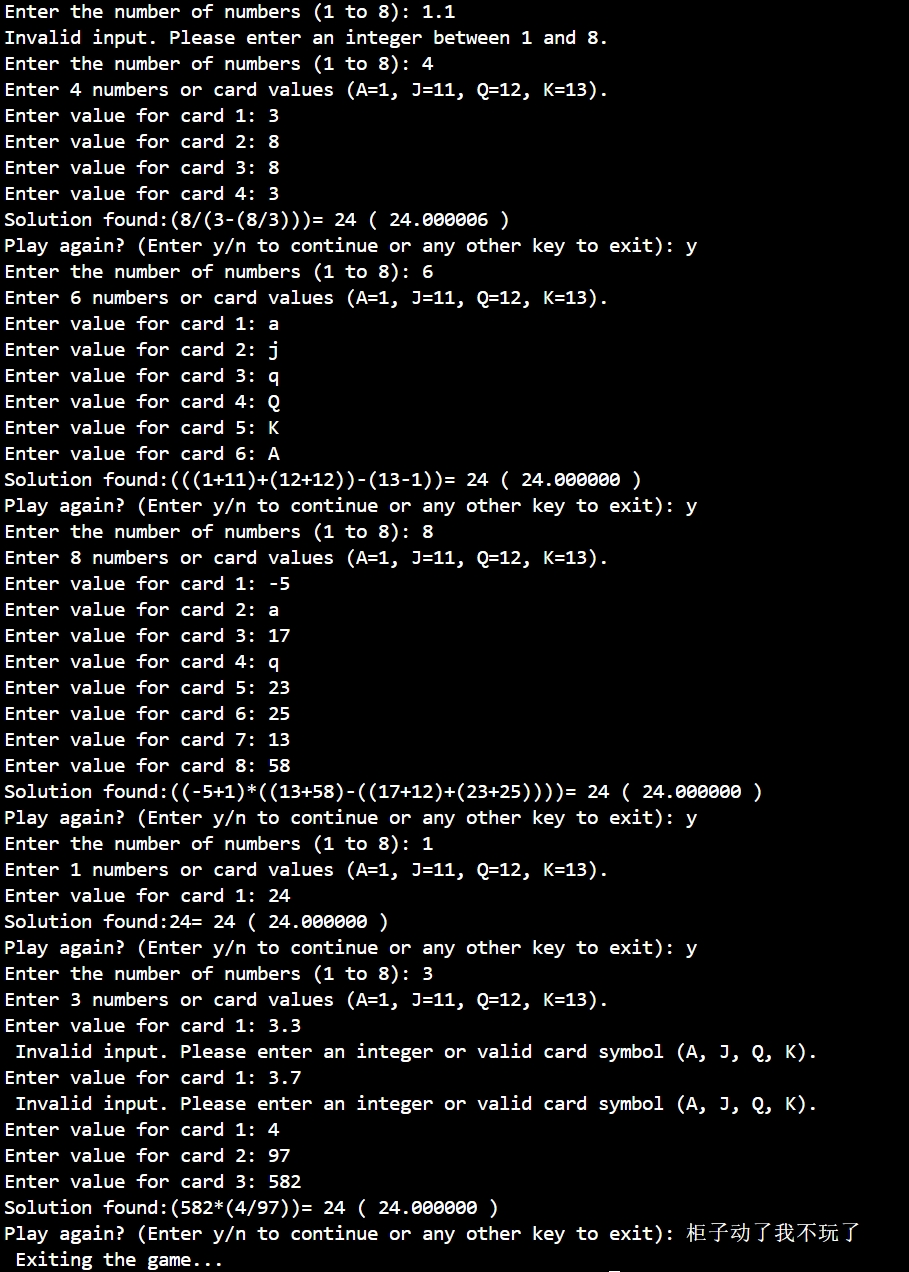
\includegraphics[width=0.9\linewidth]{Problem 2/figs/game24_promax.png}
    \caption{\texttt{Promax} 运行实例}
    \label{fig:promax}
\end{figure}

\begin{figure}[ht]
    \centering
    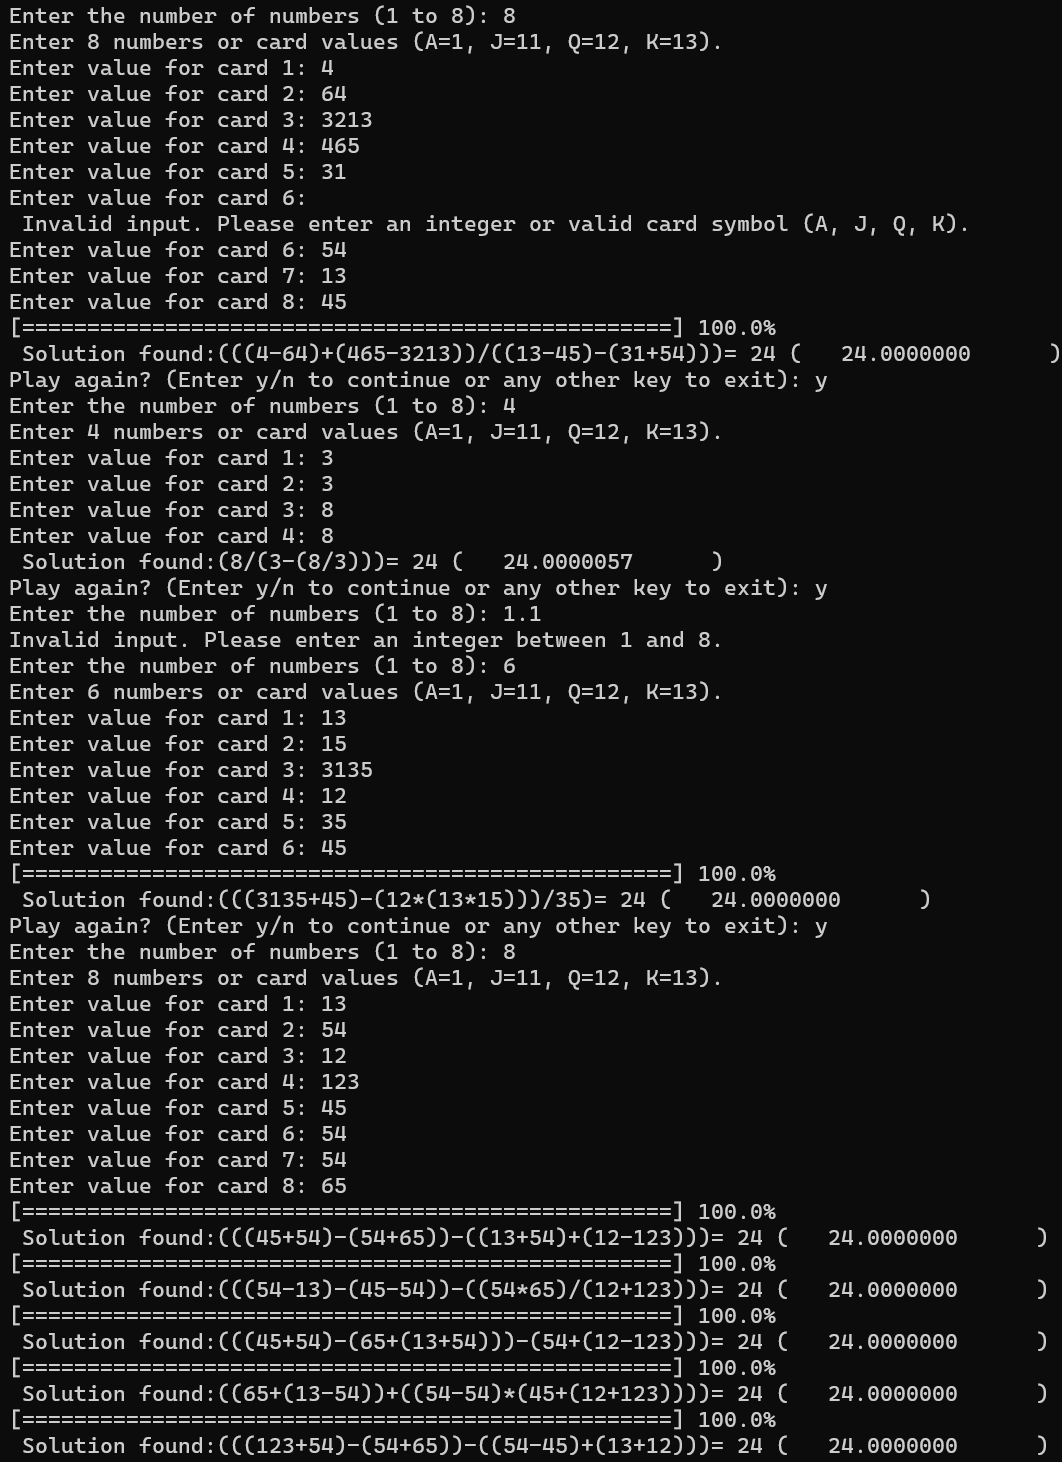
\includegraphics[width=0.9\linewidth]{Problem 2/figs/game24_ultra.png}
    \caption{\texttt{Ultra} 运行实例}
    \label{fig:Ultra}
\end{figure}




